\write18{./make_talk.sh }

\documentclass[aspectratio=169]{beamer}
\usetheme{Pittsburgh}
\usecolortheme{spruce}
\usefonttheme{structurebold}
\beamertemplatenavigationsymbolsempty
\usepackage{graphicx}
\usepackage{tikz}
\usepackage{cite}
\usepackage{pgfpages}

\setbeameroption{hide notes}
%% \input{make.out}

\title{Far Flung Forest Landscapes in the Anthropocene}
\subtitle{Structural analysis of China's embodied forest network}
\author{M.K. Lau (Ph.D.)}
\date{}
\institute{Chinese Academy of Sciences and Harvard University}


\begin{document}

\begin{frame}
  \titlepage
\end{frame}

\section*{Context}

{ % all template changes are local to this group.
    \setbeamertemplate{navigation symbols}{}
    \begin{frame}<article:0>[plain]
      \frametitle{Q \& A}
        \begin{tikzpicture}[remember picture,overlay]
            \node[at=(current page.center)] {
                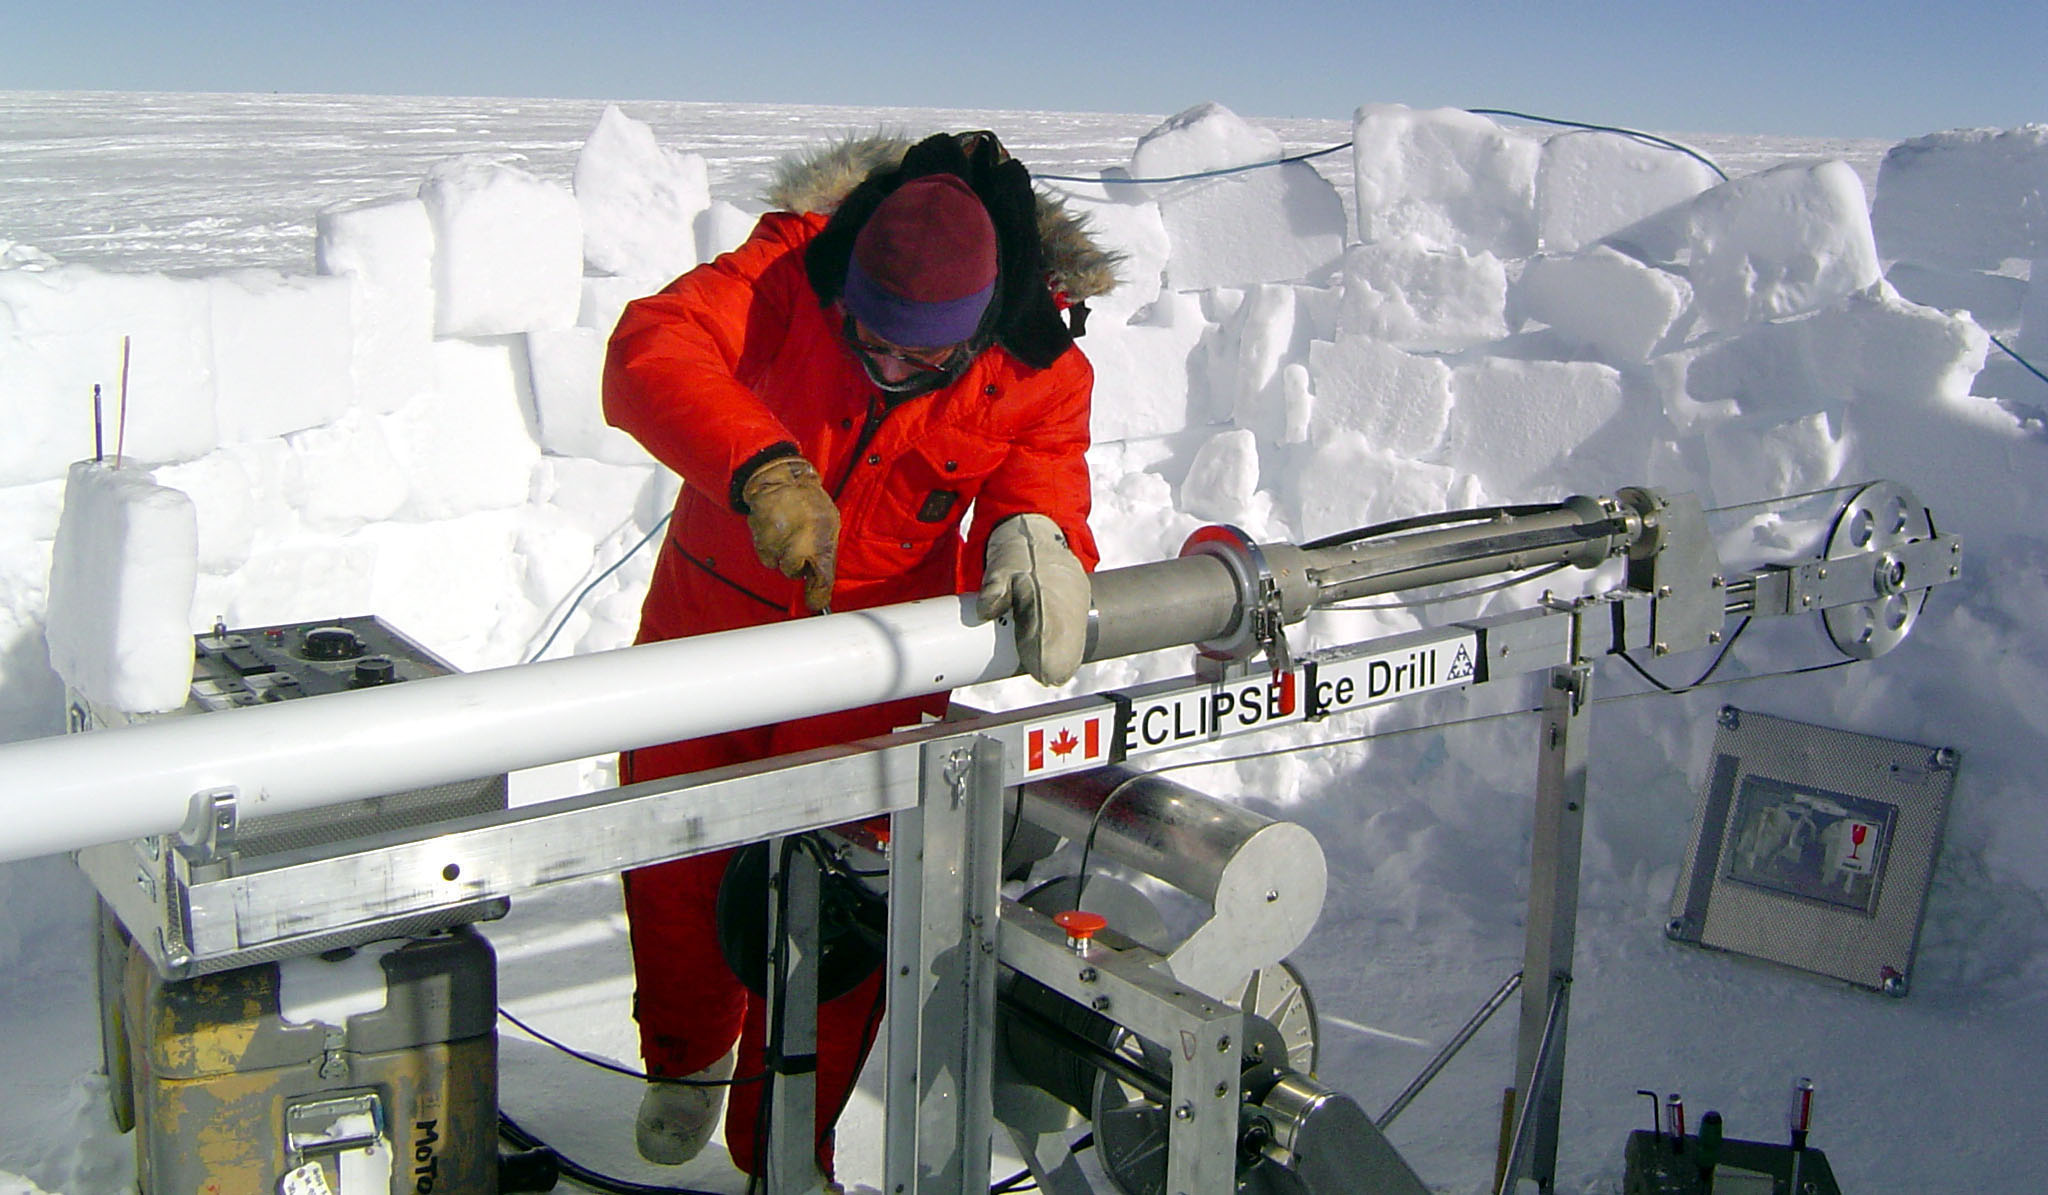
\includegraphics[keepaspectratio,
                                 width=\paperwidth]{images/ice_core.jpg}
            };
        \end{tikzpicture}
     \end{frame}
}

{ % all template changes are local to this group.
    \setbeamertemplate{navigation symbols}{}
    \begin{frame}<article:0>[plain]
      \frametitle{Q \& A}
        \begin{tikzpicture}[remember picture,overlay]
            \node[at=(current page.center)] {
                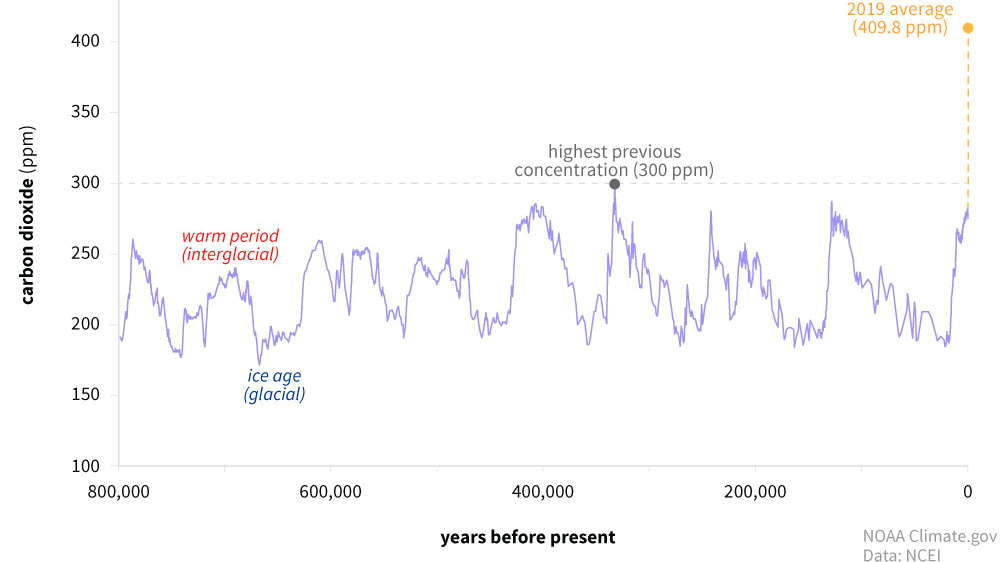
\includegraphics[keepaspectratio,
                                 width=\paperwidth]{images/BAMS_SOTC_2019_co2_paleo_1000px.jpg}
            };
        \end{tikzpicture}
     \end{frame}
}

{ % all template changes are local to this group.
    \setbeamertemplate{navigation symbols}{}
    \begin{frame}<article:0>[plain]
      \frametitle{Q \& A}
        \begin{tikzpicture}[remember picture,overlay]
            \node[at=(current page.center)] {
                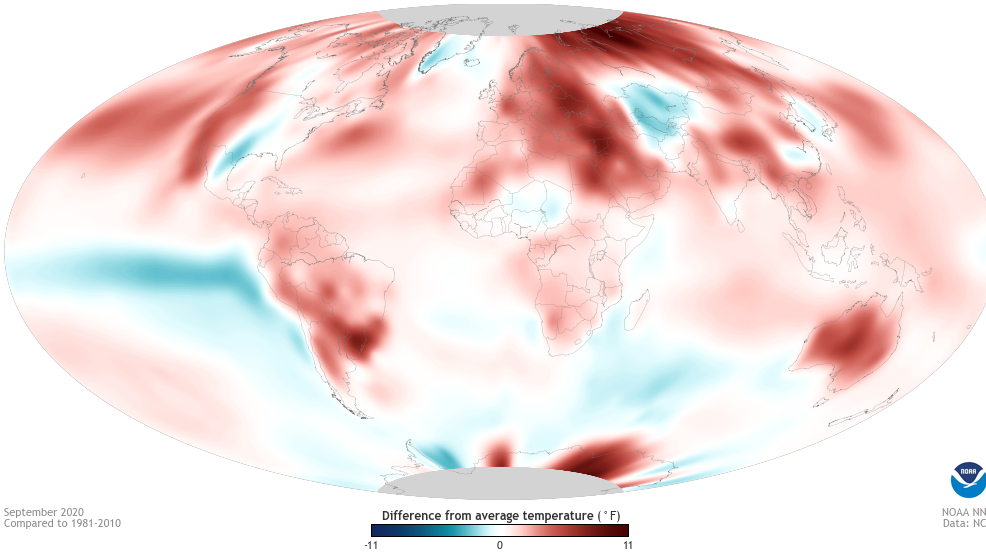
\includegraphics[keepaspectratio,
                                 width=\paperwidth]{images/September_CC2020.png}
            };
        \end{tikzpicture}
     \end{frame}
}

{ % all template changes are local to this group.
    \setbeamertemplate{navigation symbols}{}
    \begin{frame}<article:0>[plain]
      \frametitle{Q \& A}
      \cite{Ellis2020AnthropogenicCE}
        \begin{tikzpicture}[remember picture,overlay]
            \node[at=(current page.center)] {
                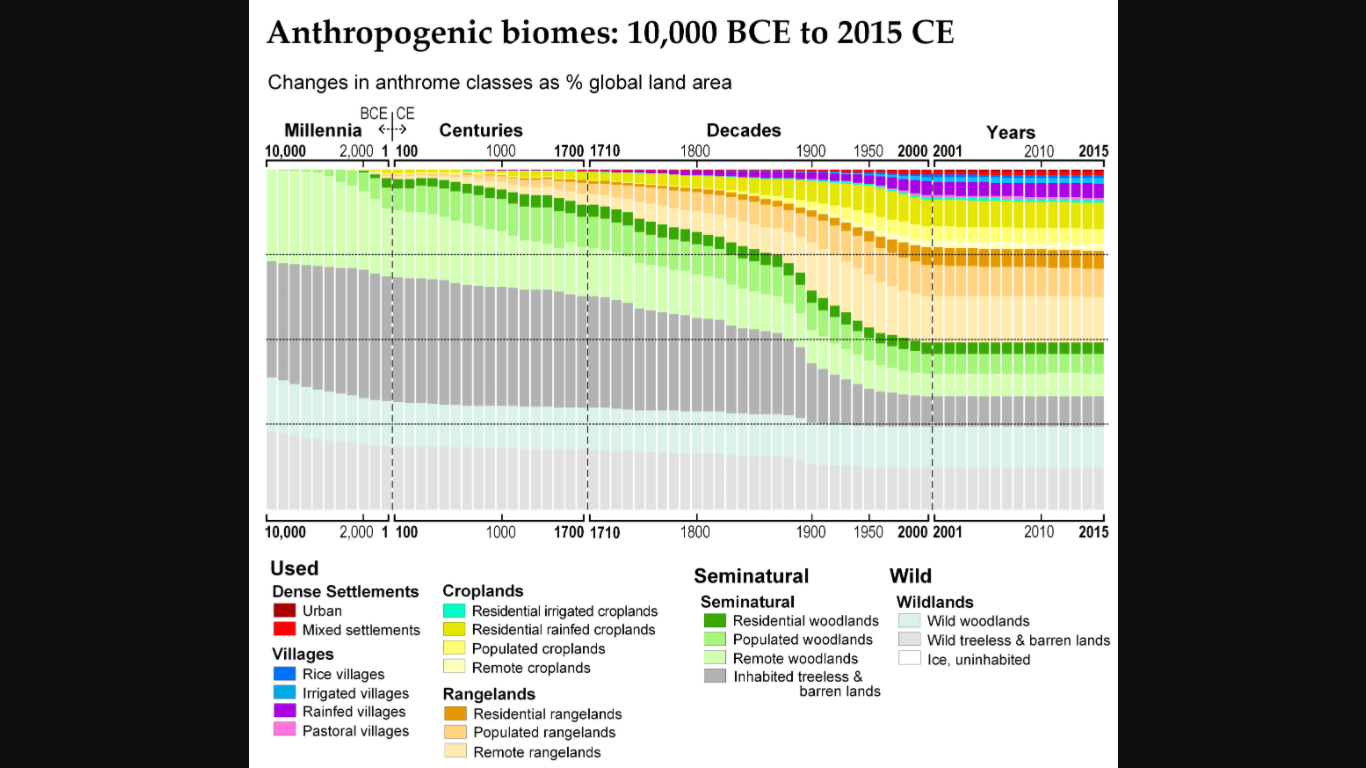
\includegraphics[keepaspectratio,
                                 width=\paperwidth,
                                 scale=0.25]{images/anthromes.png}
            };
        \end{tikzpicture}
     \end{frame}
}

{ % all template changes are local to this group.
    \setbeamertemplate{navigation symbols}{}
    \begin{frame}<article:0>[plain]
      \frametitle{Q \& A}
        \begin{tikzpicture}[remember picture,overlay]
            \node[at=(current page.center)] {
                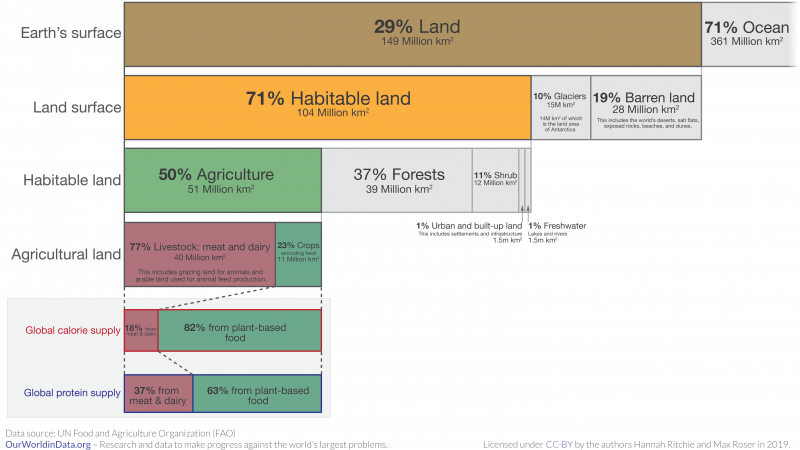
\includegraphics[keepaspectratio,
                                 width=\paperwidth,
                                 scale=0.25]{images/Global-land-use-graphic-800x506.png}
            };
        \end{tikzpicture}
     \end{frame}
}


{ % all template changes are local to this group.
    \setbeamertemplate{navigation symbols}{}
    \begin{frame}<article:0>[plain]
      \frametitle{Q \& A}
        \begin{tikzpicture}[remember picture,overlay]
            \node[at=(current page.center)] {
                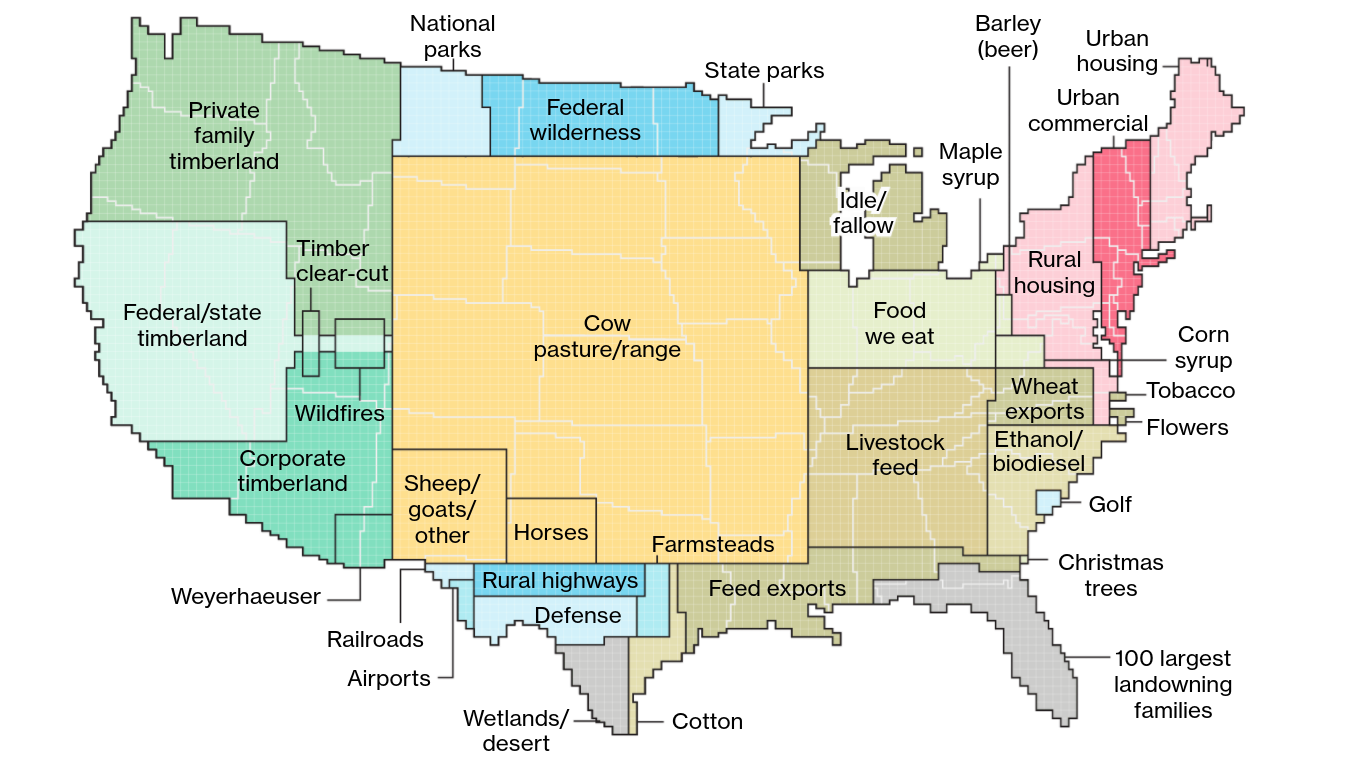
\includegraphics[keepaspectratio,
                                 width=\paperwidth]{images/how-america-uses-its-land.png}
            };
        \end{tikzpicture}
     \end{frame}
}



\begin{frame}
  \frametitle{Forests in the Anthropocence}

  \note[item]{Anthropocene = proposed geological epoch distinguished by human impacts}
  \note[item]{One proposal is it started about 1950 with acceleration}
  \note[item]{90\% biomass on Earth is humans and livestock}
  \note[item]{Atmospheric changes}
  \note[item]{Land-use changes}
  \note[item]{Biodiversity changes}
  
\end{frame}


{ % all template changes are local to this group.
    \setbeamertemplate{navigation symbols}{}
    \begin{frame}<article:0>[plain]
      \frametitle{Q \& A}
        \begin{tikzpicture}[remember picture,overlay]
            \node[at=(current page.center)] {
                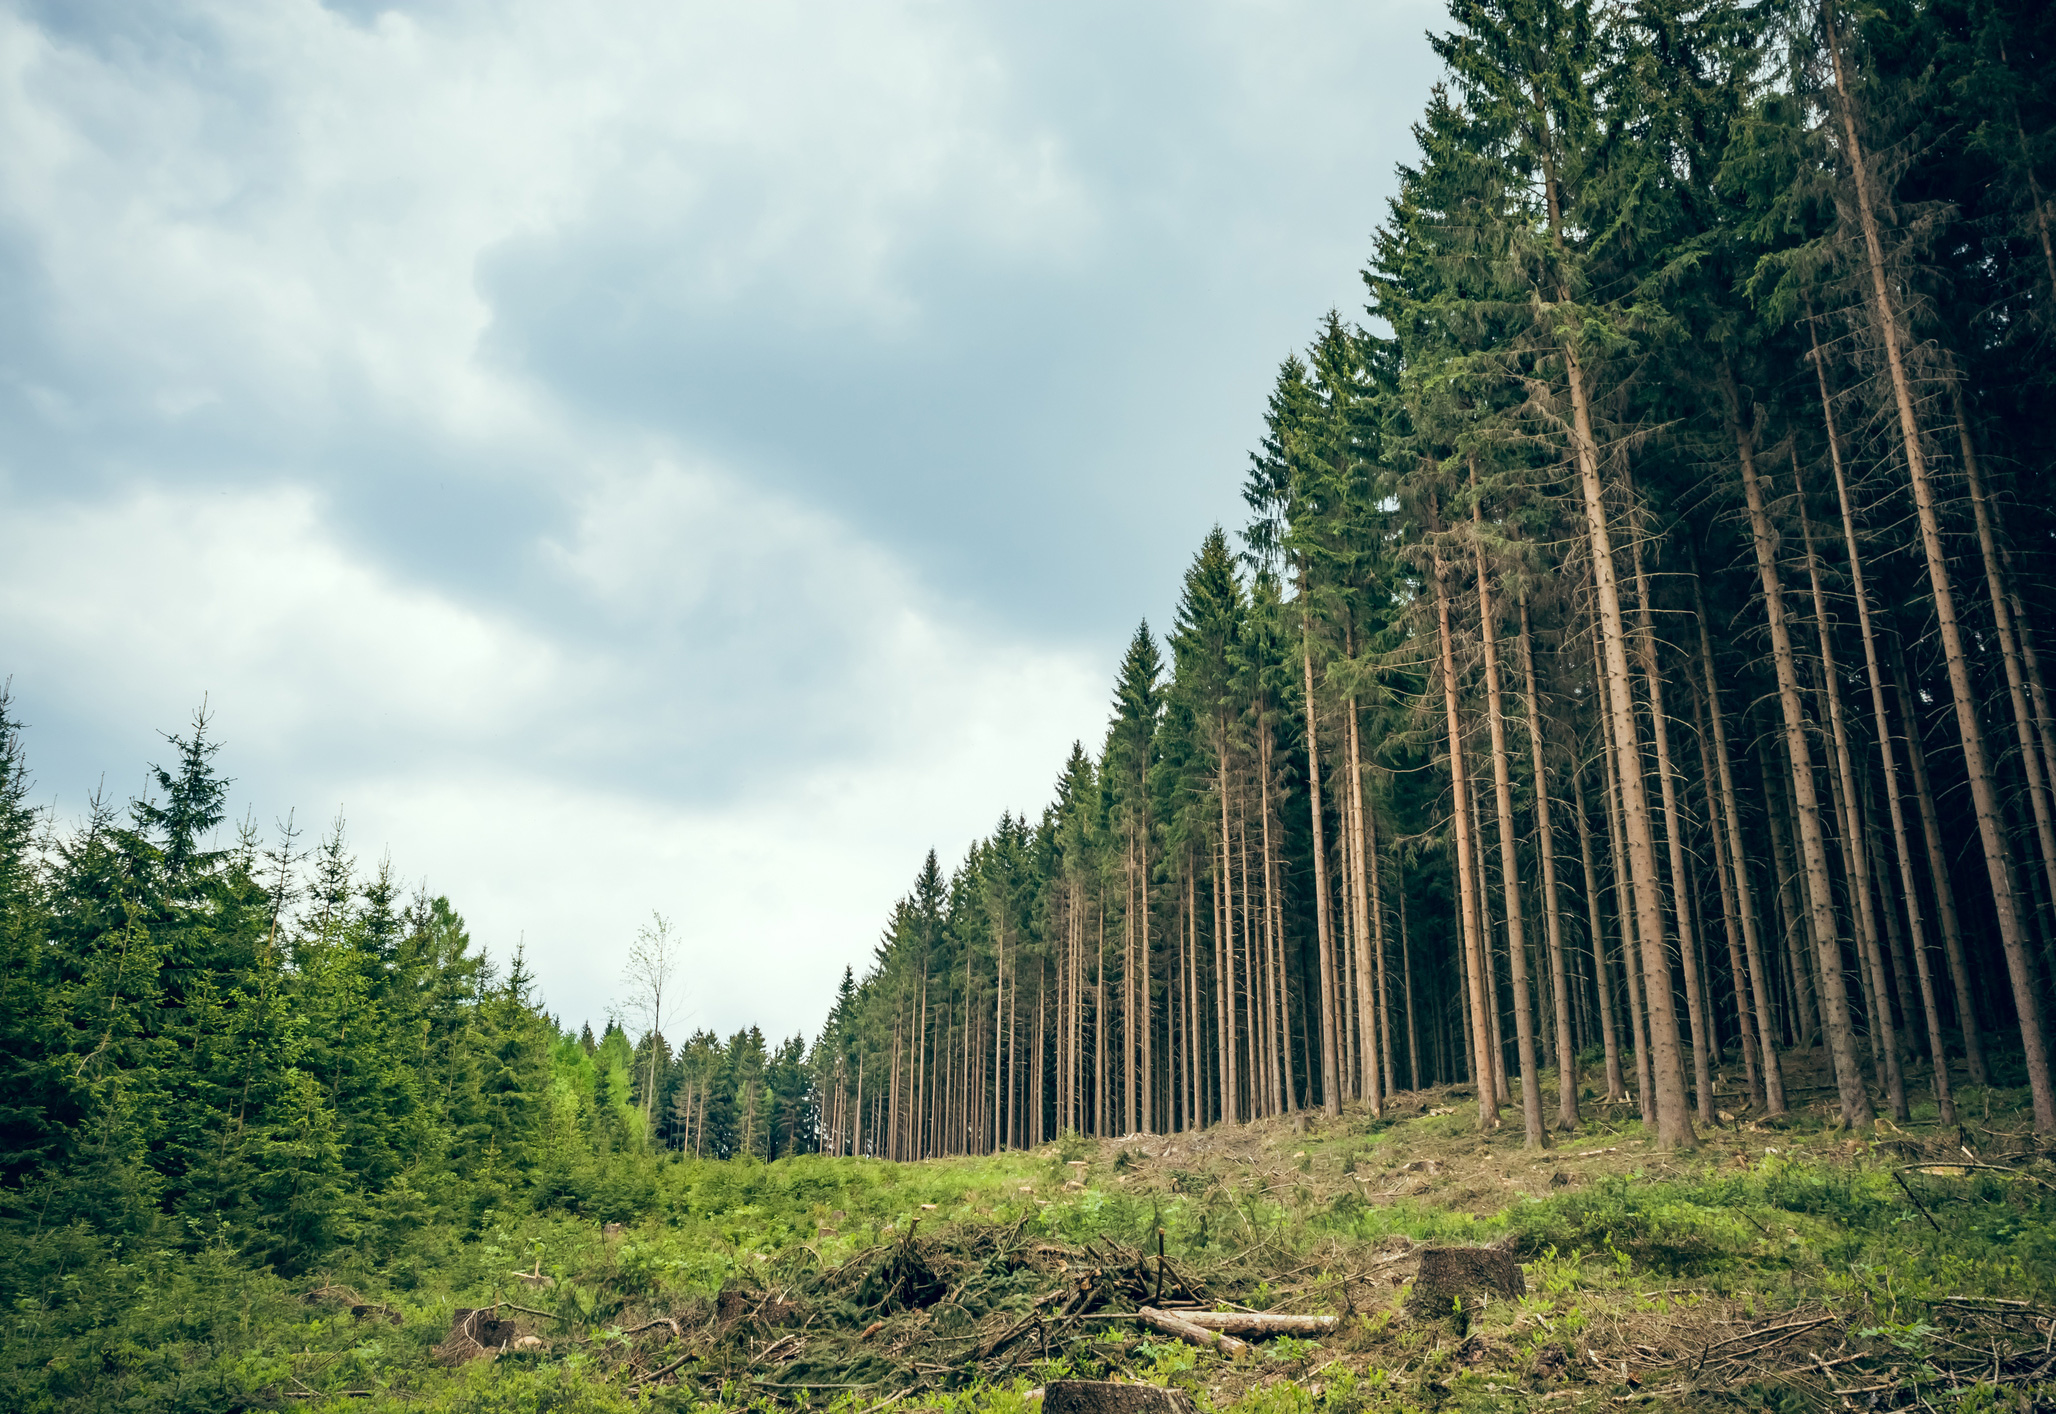
\includegraphics[keepaspectratio,
                                 width=\paperwidth]{images/forest-cut.jpg}
            };
        \end{tikzpicture}
     \end{frame}
}

{ % all template changes are local to this group.
    \setbeamertemplate{navigation symbols}{}
    \begin{frame}<article:0>[plain]
      \frametitle{Q \& A}
        \begin{tikzpicture}[remember picture,overlay]
            \node[at=(current page.center)] {
                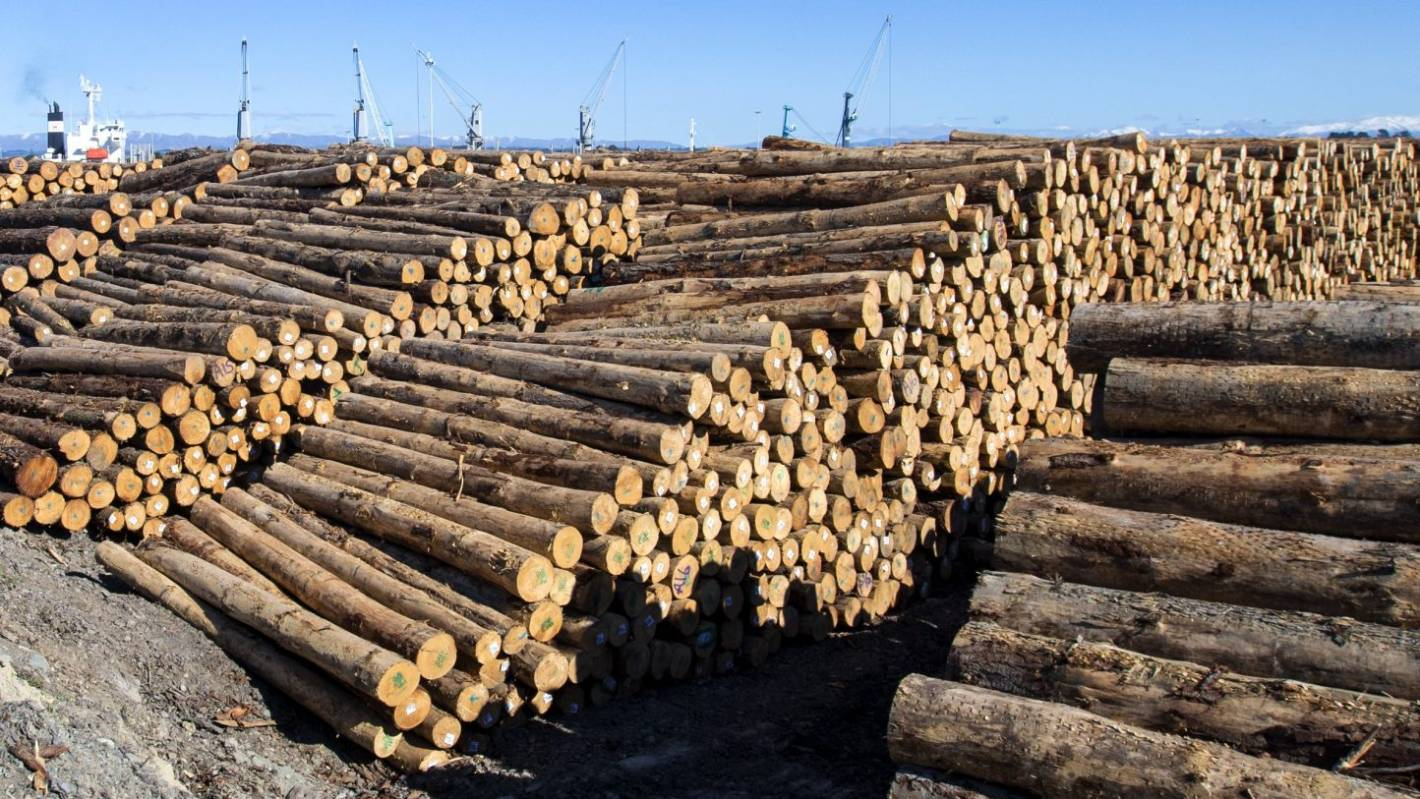
\includegraphics[keepaspectratio,
                                 width=\paperwidth]{images/sawn-logs.jpg}
            };
        \end{tikzpicture}
     \end{frame}
}


\begin{frame}
  \frametitle{Forests are Important}

  \begin{itemize}
  \item Carbon Storage \pause
  \item Water and nutrient cycling \pause
  \item Resources \pause
  \item Biodiversity \pause
  \item Human Health and Culture 
  \end{itemize}

\end{frame}



{ % all template changes are local to this group.
    \setbeamertemplate{navigation symbols}{}
    \begin{frame}<article:0>[plain]
      \frametitle{Q \& A}
        \begin{tikzpicture}[remember picture,overlay]
            \node[at=(current page.center)] {
                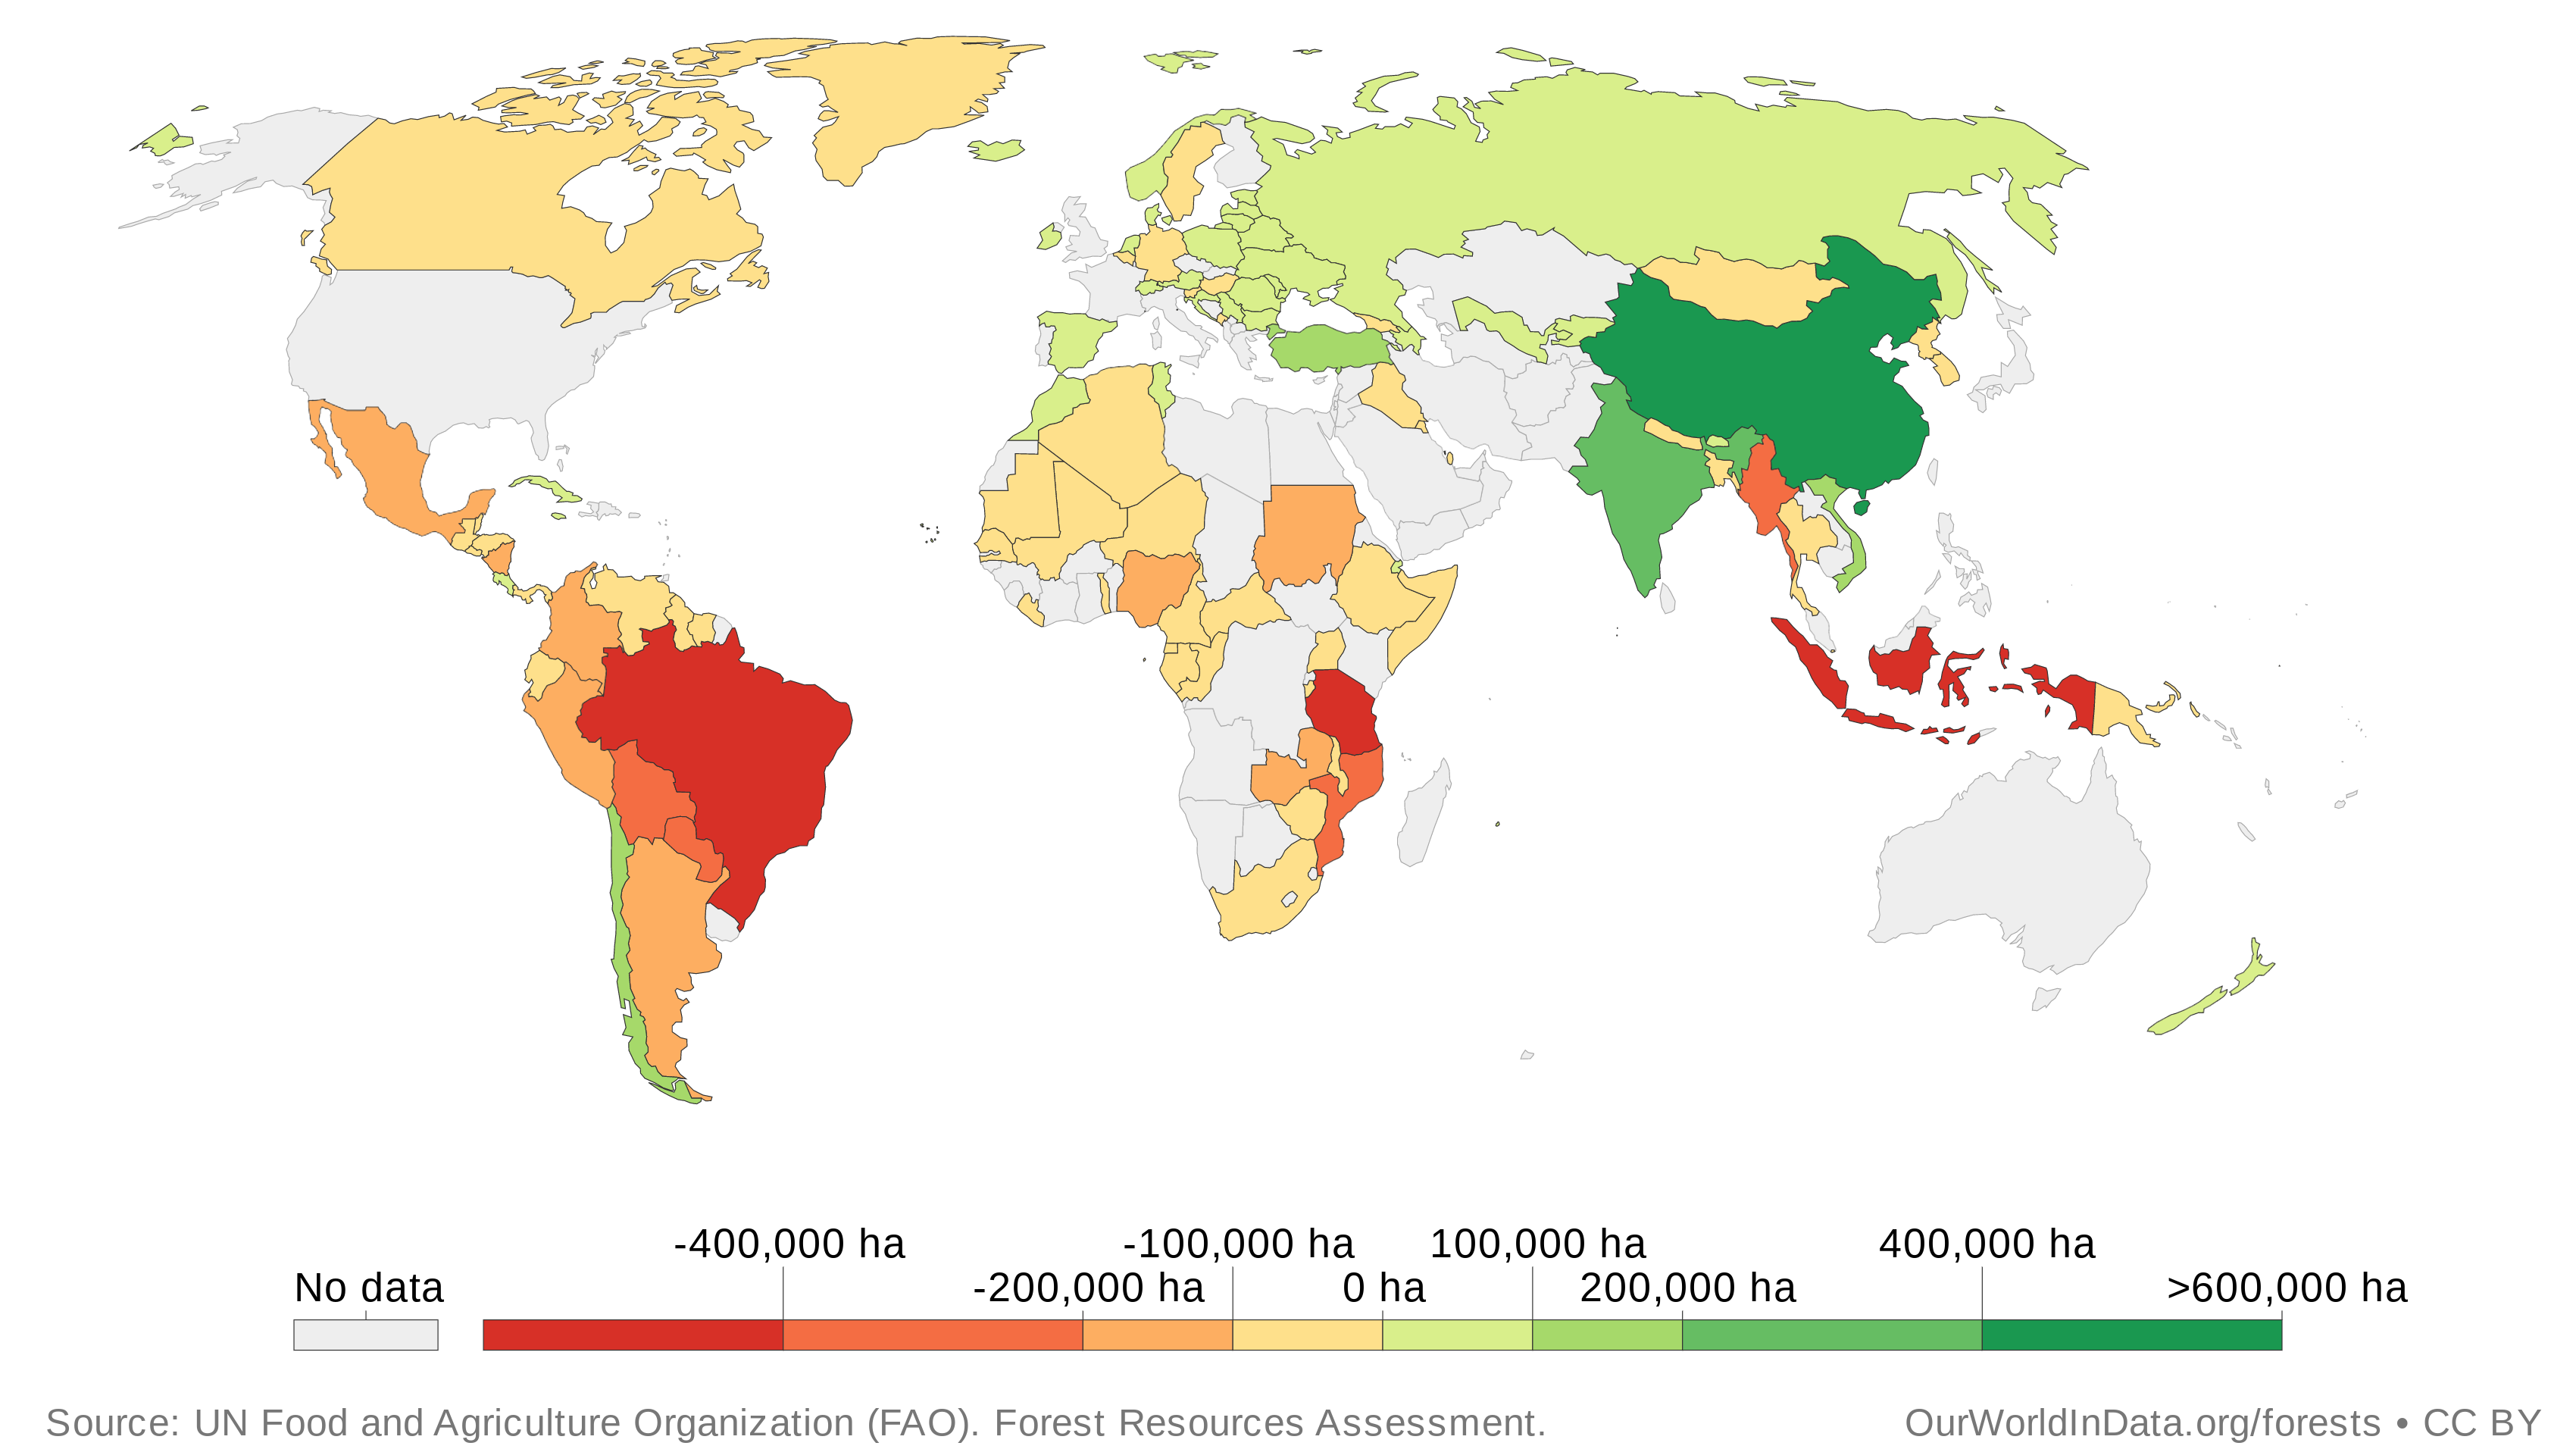
\includegraphics[keepaspectratio,
                                 width=\paperwidth]{images/annual-change-forest-area.png}
            };
        \end{tikzpicture}
     \end{frame}
}



{ % all template changes are local to this group.
    \setbeamertemplate{navigation symbols}{}
    \begin{frame}<article:0>[plain]
      \frametitle{Q \& A}
        \begin{tikzpicture}[remember picture,overlay]
            \node[at=(current page.center)] {
                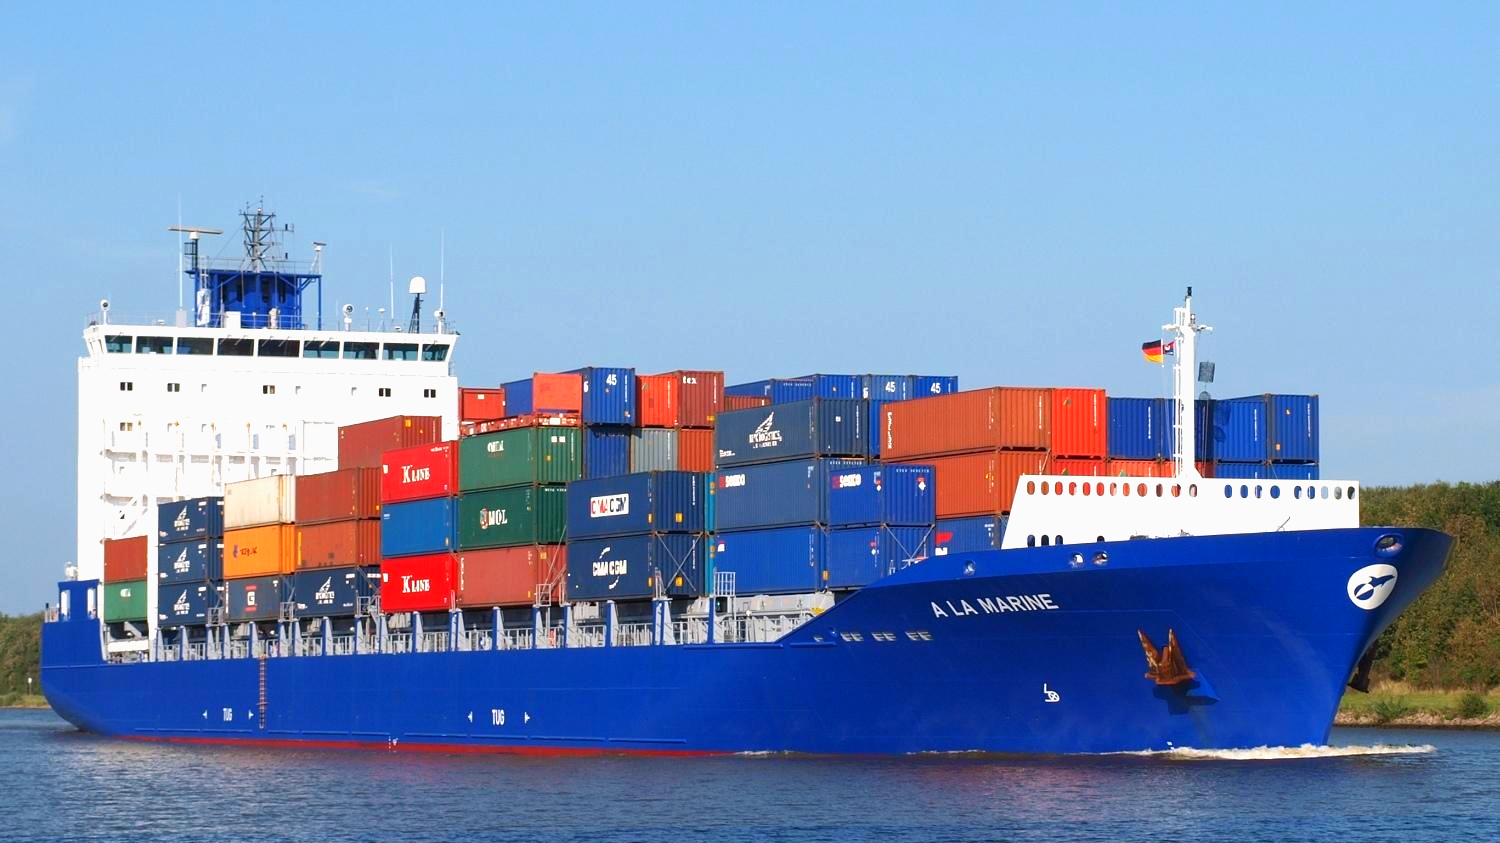
\includegraphics[keepaspectratio,
                                 width=\paperwidth]{images/shipping-ship.jpg}
            };
        \end{tikzpicture}
     \end{frame}
}


{ % all template changes are local to this group.
    \setbeamertemplate{navigation symbols}{}
    \begin{frame}<article:0>[plain]
      \frametitle{Q \& A}
        \begin{tikzpicture}[remember picture,overlay]
            \node[at=(current page.center)] {
                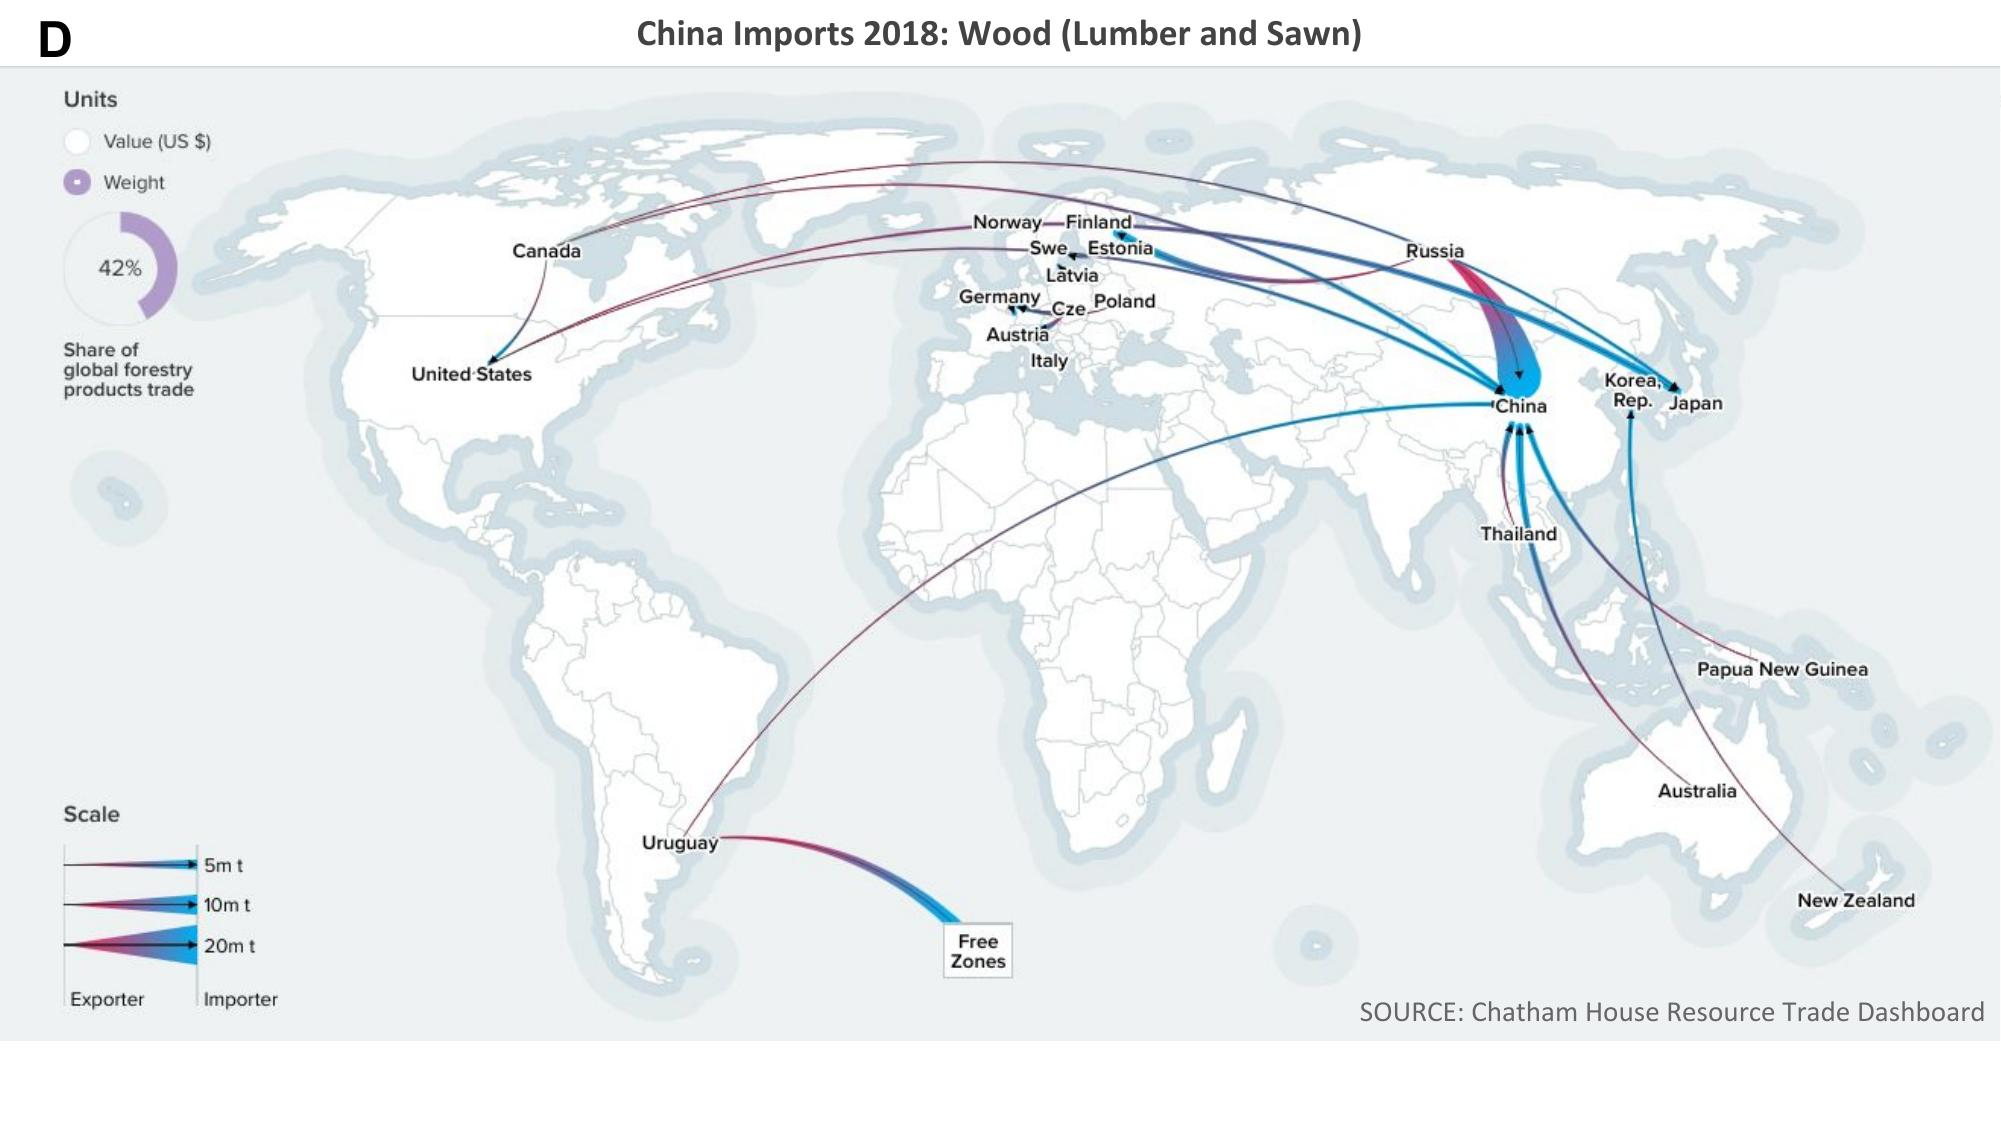
\includegraphics[keepaspectratio,
                                 width=\paperwidth]{images/resourcetrade_network.jpeg}
            };
        \end{tikzpicture}
     \end{frame}
}


\begin{frame}
  \frametitle{Forests in the Anthropocence}
  
  \begin{itemize}
  \item Forests are changing from human impacts \pause
  \item Large direct effects of land-use  \pause
  \item How do we address indirect and systems-level effects? 
  \end{itemize}

\end{frame}


\begin{frame}
  \frametitle{Today's Talk}

\tableofcontents

\note[item]{- Intro/Context}
\note[item]{  - Forests are globally important}
\note[item]{  - Anthropocence effects }
\note[item]{  - Global forest loss and gain and change}
\note[item]{	- Global greening = India(Agriculture) + China(Forests)}
\note[item]{- Economics*Ecology = Landscape Extended Models}
\note[item]{- Network Analysis of China's Greening}
\note[item]{  - Global Scale}
\note[item]{  - Local Scale}
\note[item]{	- Landscape = Chen 2019}
\note[item]{	- Resilience Analysis of China's Forest LE-MRIO}
\note[item]{- Conclusions and Future Work}
\note[item]{- Acknowledgements}

\end{frame}



\section{Economic and Ecological Landscape Extensions}

\begin{frame}
  \frametitle{Economic and Ecological Landscape Extensions}
\end{frame}

  %% - Global forest loss and gain and change
  %% - Global greening = India(Agriculture) + China(Forests)


\section{Trade Networks of Forest Landscapes}

\begin{frame}
  \frametitle{Trade Networks of Forest Landscapes}
\end{frame}



\section{Global Forest Networks}

\begin{frame}
  \frametitle{Global Forest Networks}
\end{frame}


\section{China's Forest Networks: Global}

\begin{frame}
  \frametitle{China's Forest Networks: Global}
\end{frame}


\section{China's Forest Networks: Domestic/Local}

\begin{frame}
  \frametitle{China's Forest Networks: Domestic/Local}
\end{frame}

%%   - Local Scale
%% 	- Landscape = Chen 2019
%% 	- Resilience Analysis of China's Forest LE-MRIO

\section{Conclusions}

\begin{frame}
  \frametitle{Conclusions}
\end{frame}

\section{Future Work}

\begin{frame}
  \frametitle{Future Work}
\end{frame}

\begin{frame}
  \frametitle{Acknowledgements}
\end{frame}



{ % all template changes are local to this group.
    \setbeamertemplate{navigation symbols}{}
    \begin{frame}<article:0>[plain]
      \frametitle{Q \& A}
        \begin{tikzpicture}[remember picture,overlay]
            \node[at=(current page.center)] {
                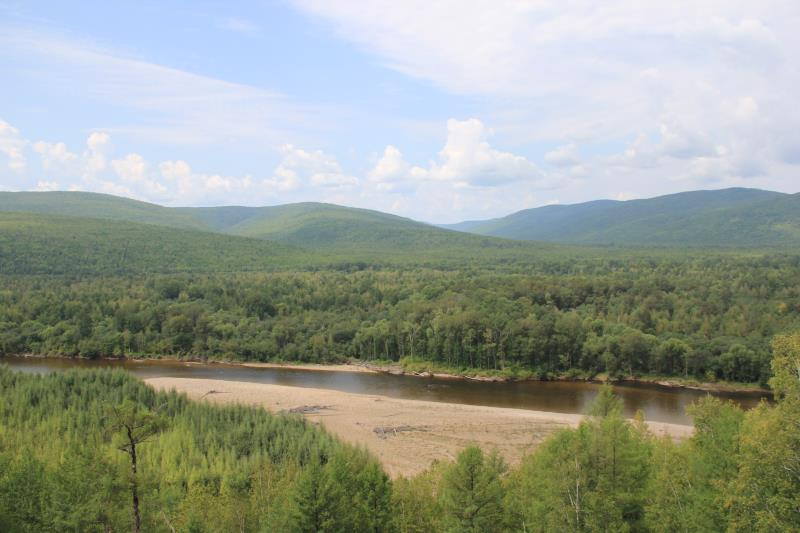
\includegraphics[keepaspectratio,
                                 width=\paperwidth]{images/CNF/IMG_0199.JPG}
            };
        \end{tikzpicture}
     \end{frame}
}

\begin{frame}
  \cite{Burgess2012}    
  \cite{Caggiani2014}
  \cite{Carvalho2019AdaptationSystems}
  \cite{Schaffer-Smith2018NetworkTrade}
\end{frame}


\begin{frame}[allowframebreaks]
  \frametitle{References}
  \tiny \bibliography{biblio.bib}
  \bibliographystyle{abbrv}
\end{frame}


\end{document}
